\section{Applying deep learning models to joins}
\label{join_system}

%\begin{figure*}[htb]
%    \centering
%    \begin{subfigure}[t]{0.24\linewidth}
%        \centering
%        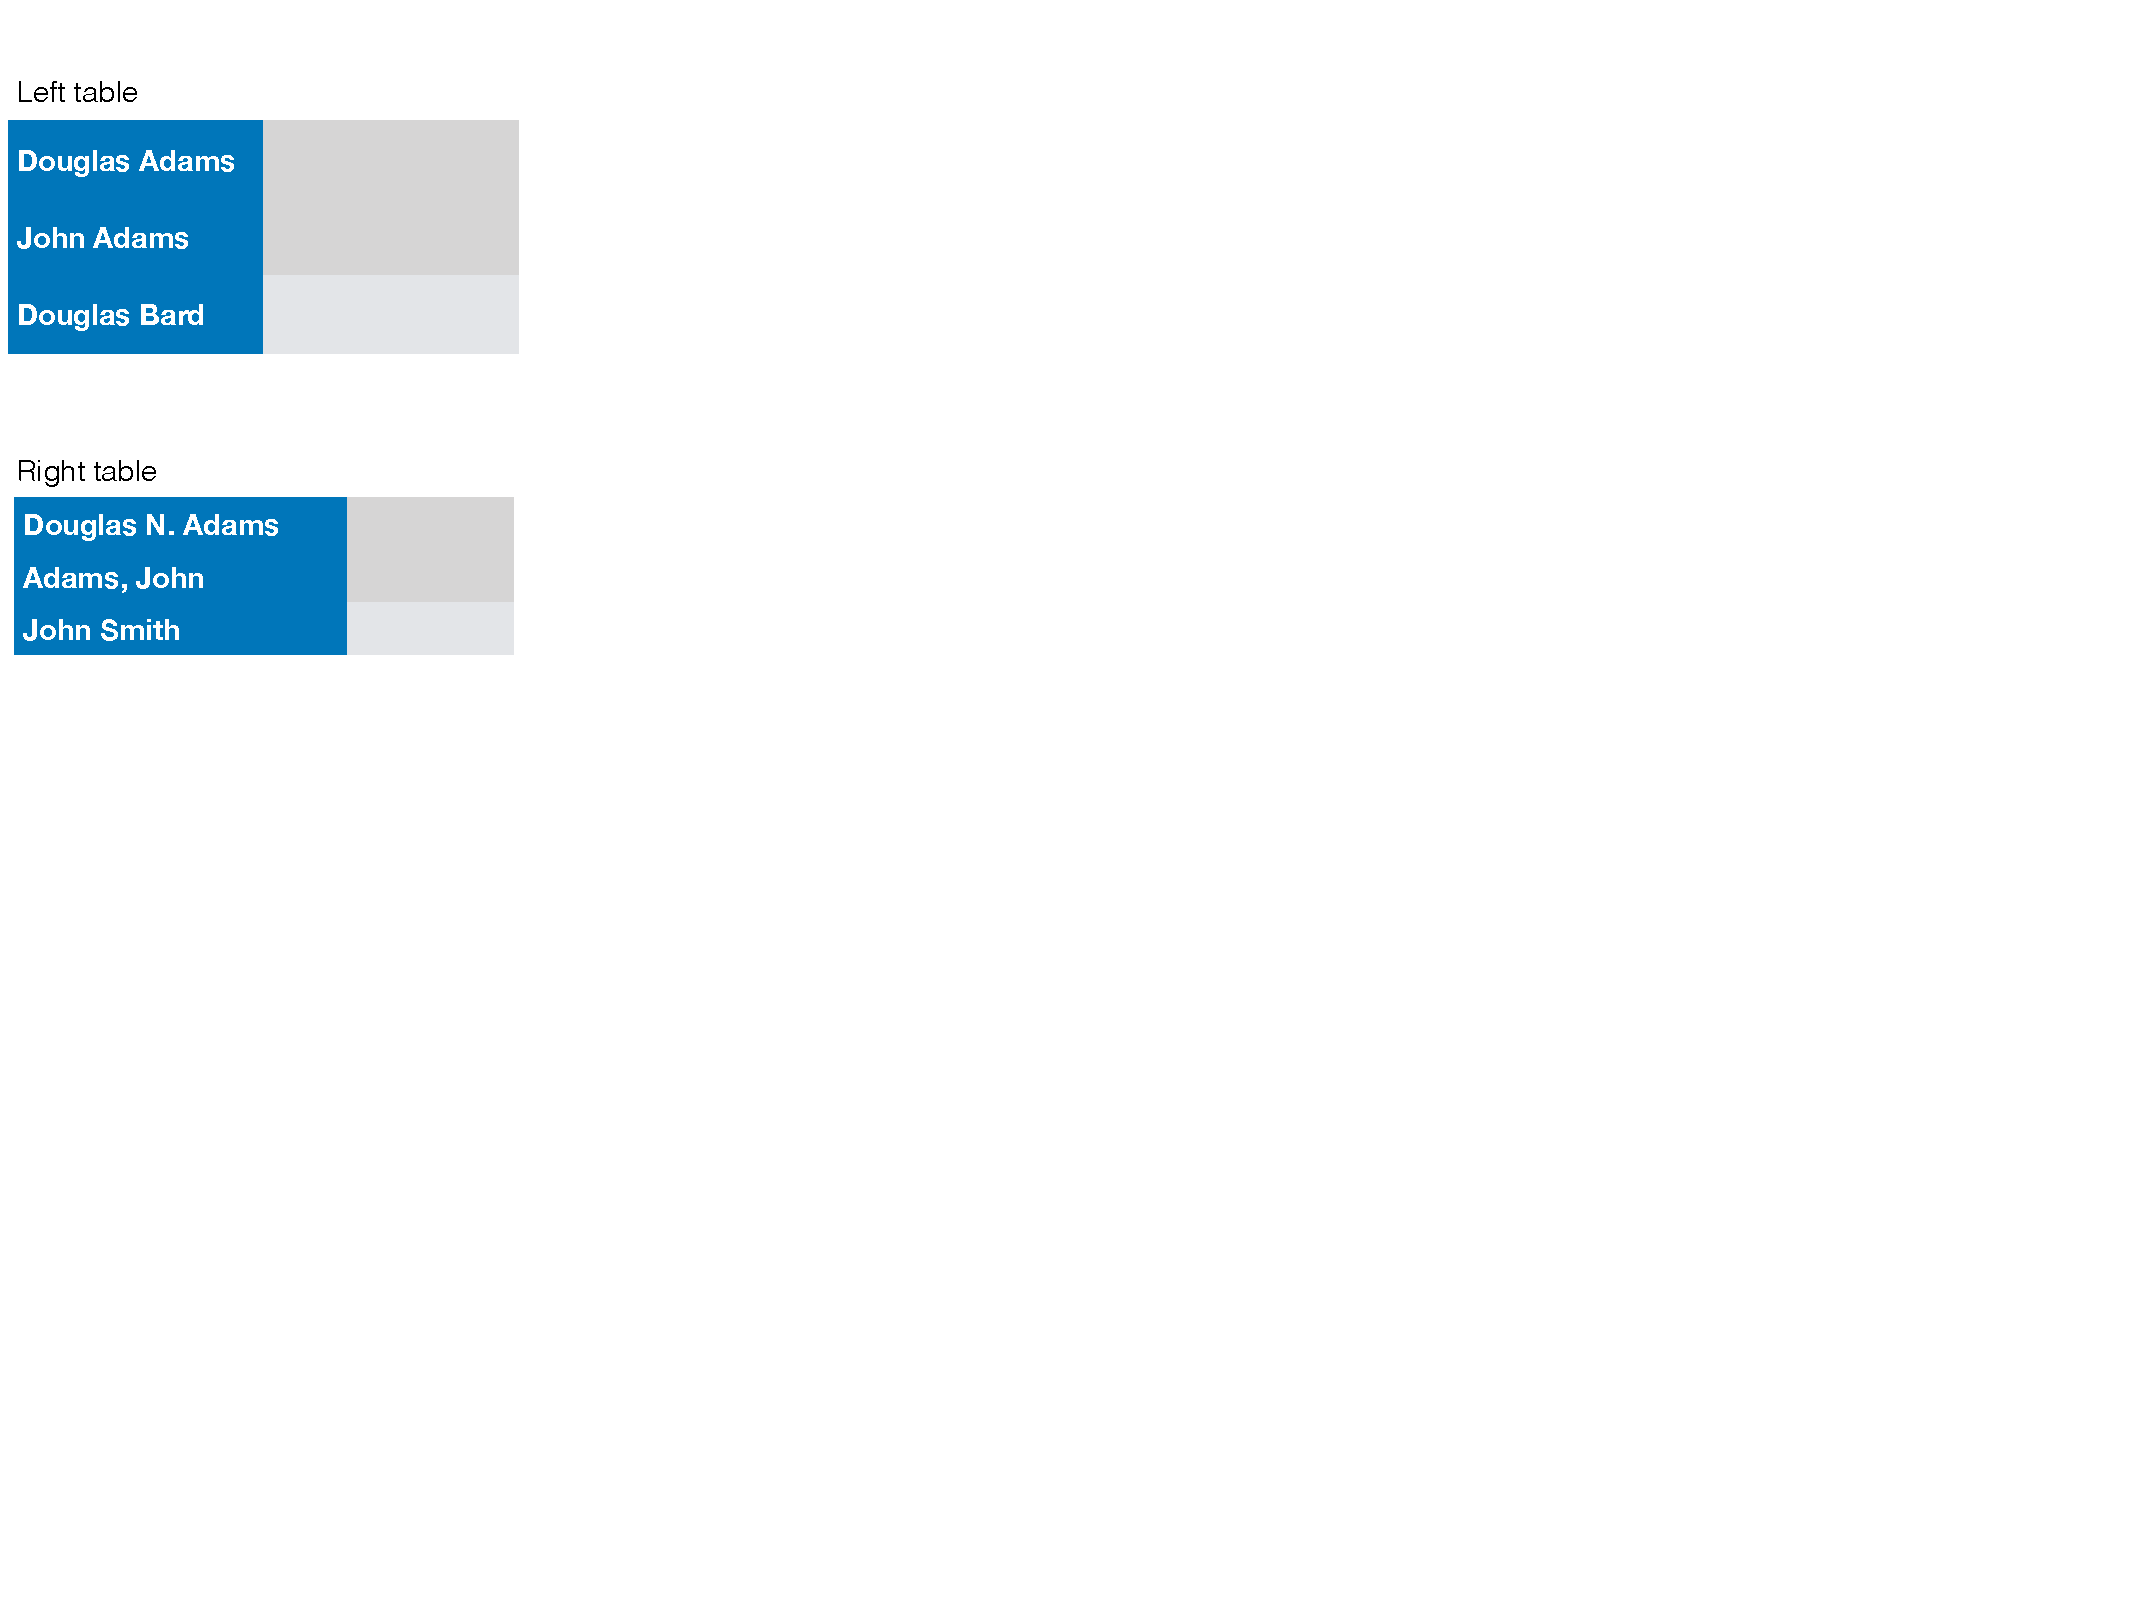
\includegraphics[width=.9\linewidth]{join1}
%        \caption{Columns to be merged}
%        \label{join1}
%    \end{subfigure}%
%    ~ 
%    \begin{subfigure}[t]{0.24\linewidth}
%        \centering 
%        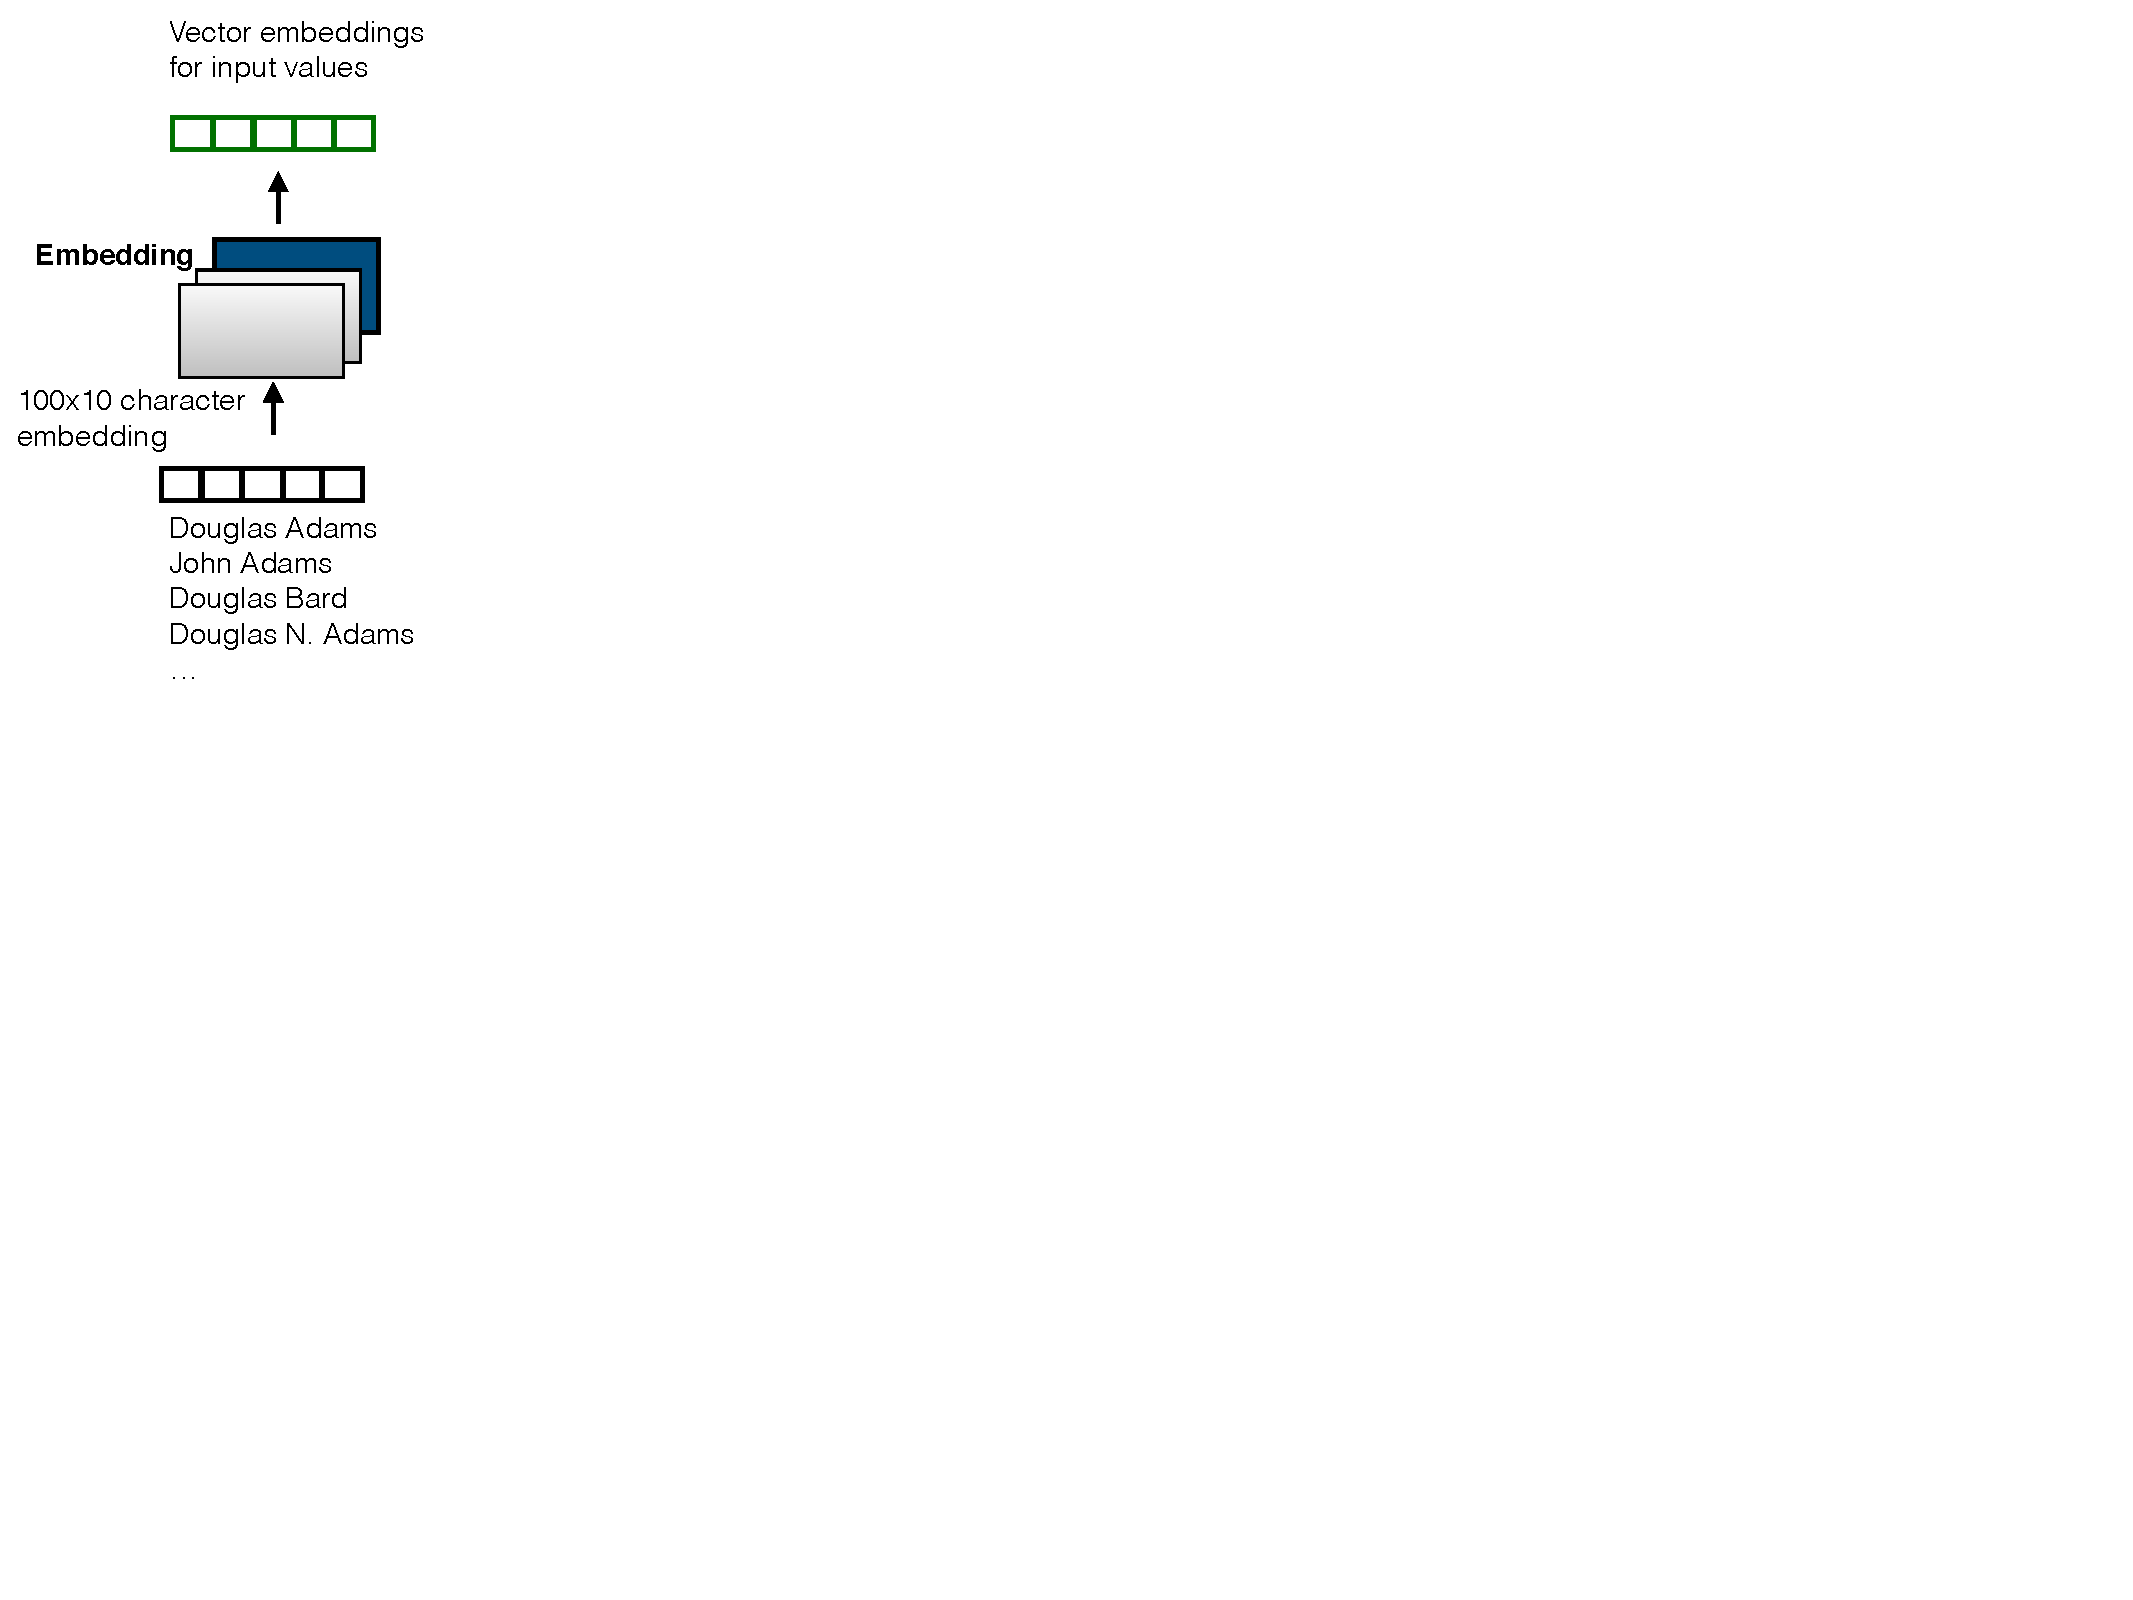
\includegraphics[width=.9\linewidth]{join2}
%        \caption{Create embeddings for each cell value in each column using the siamese model}
%        \label{join2}
%    \end{subfigure}
%    ~ 
%    \begin{subfigure}[t]{0.24\linewidth}
%        \centering 
%        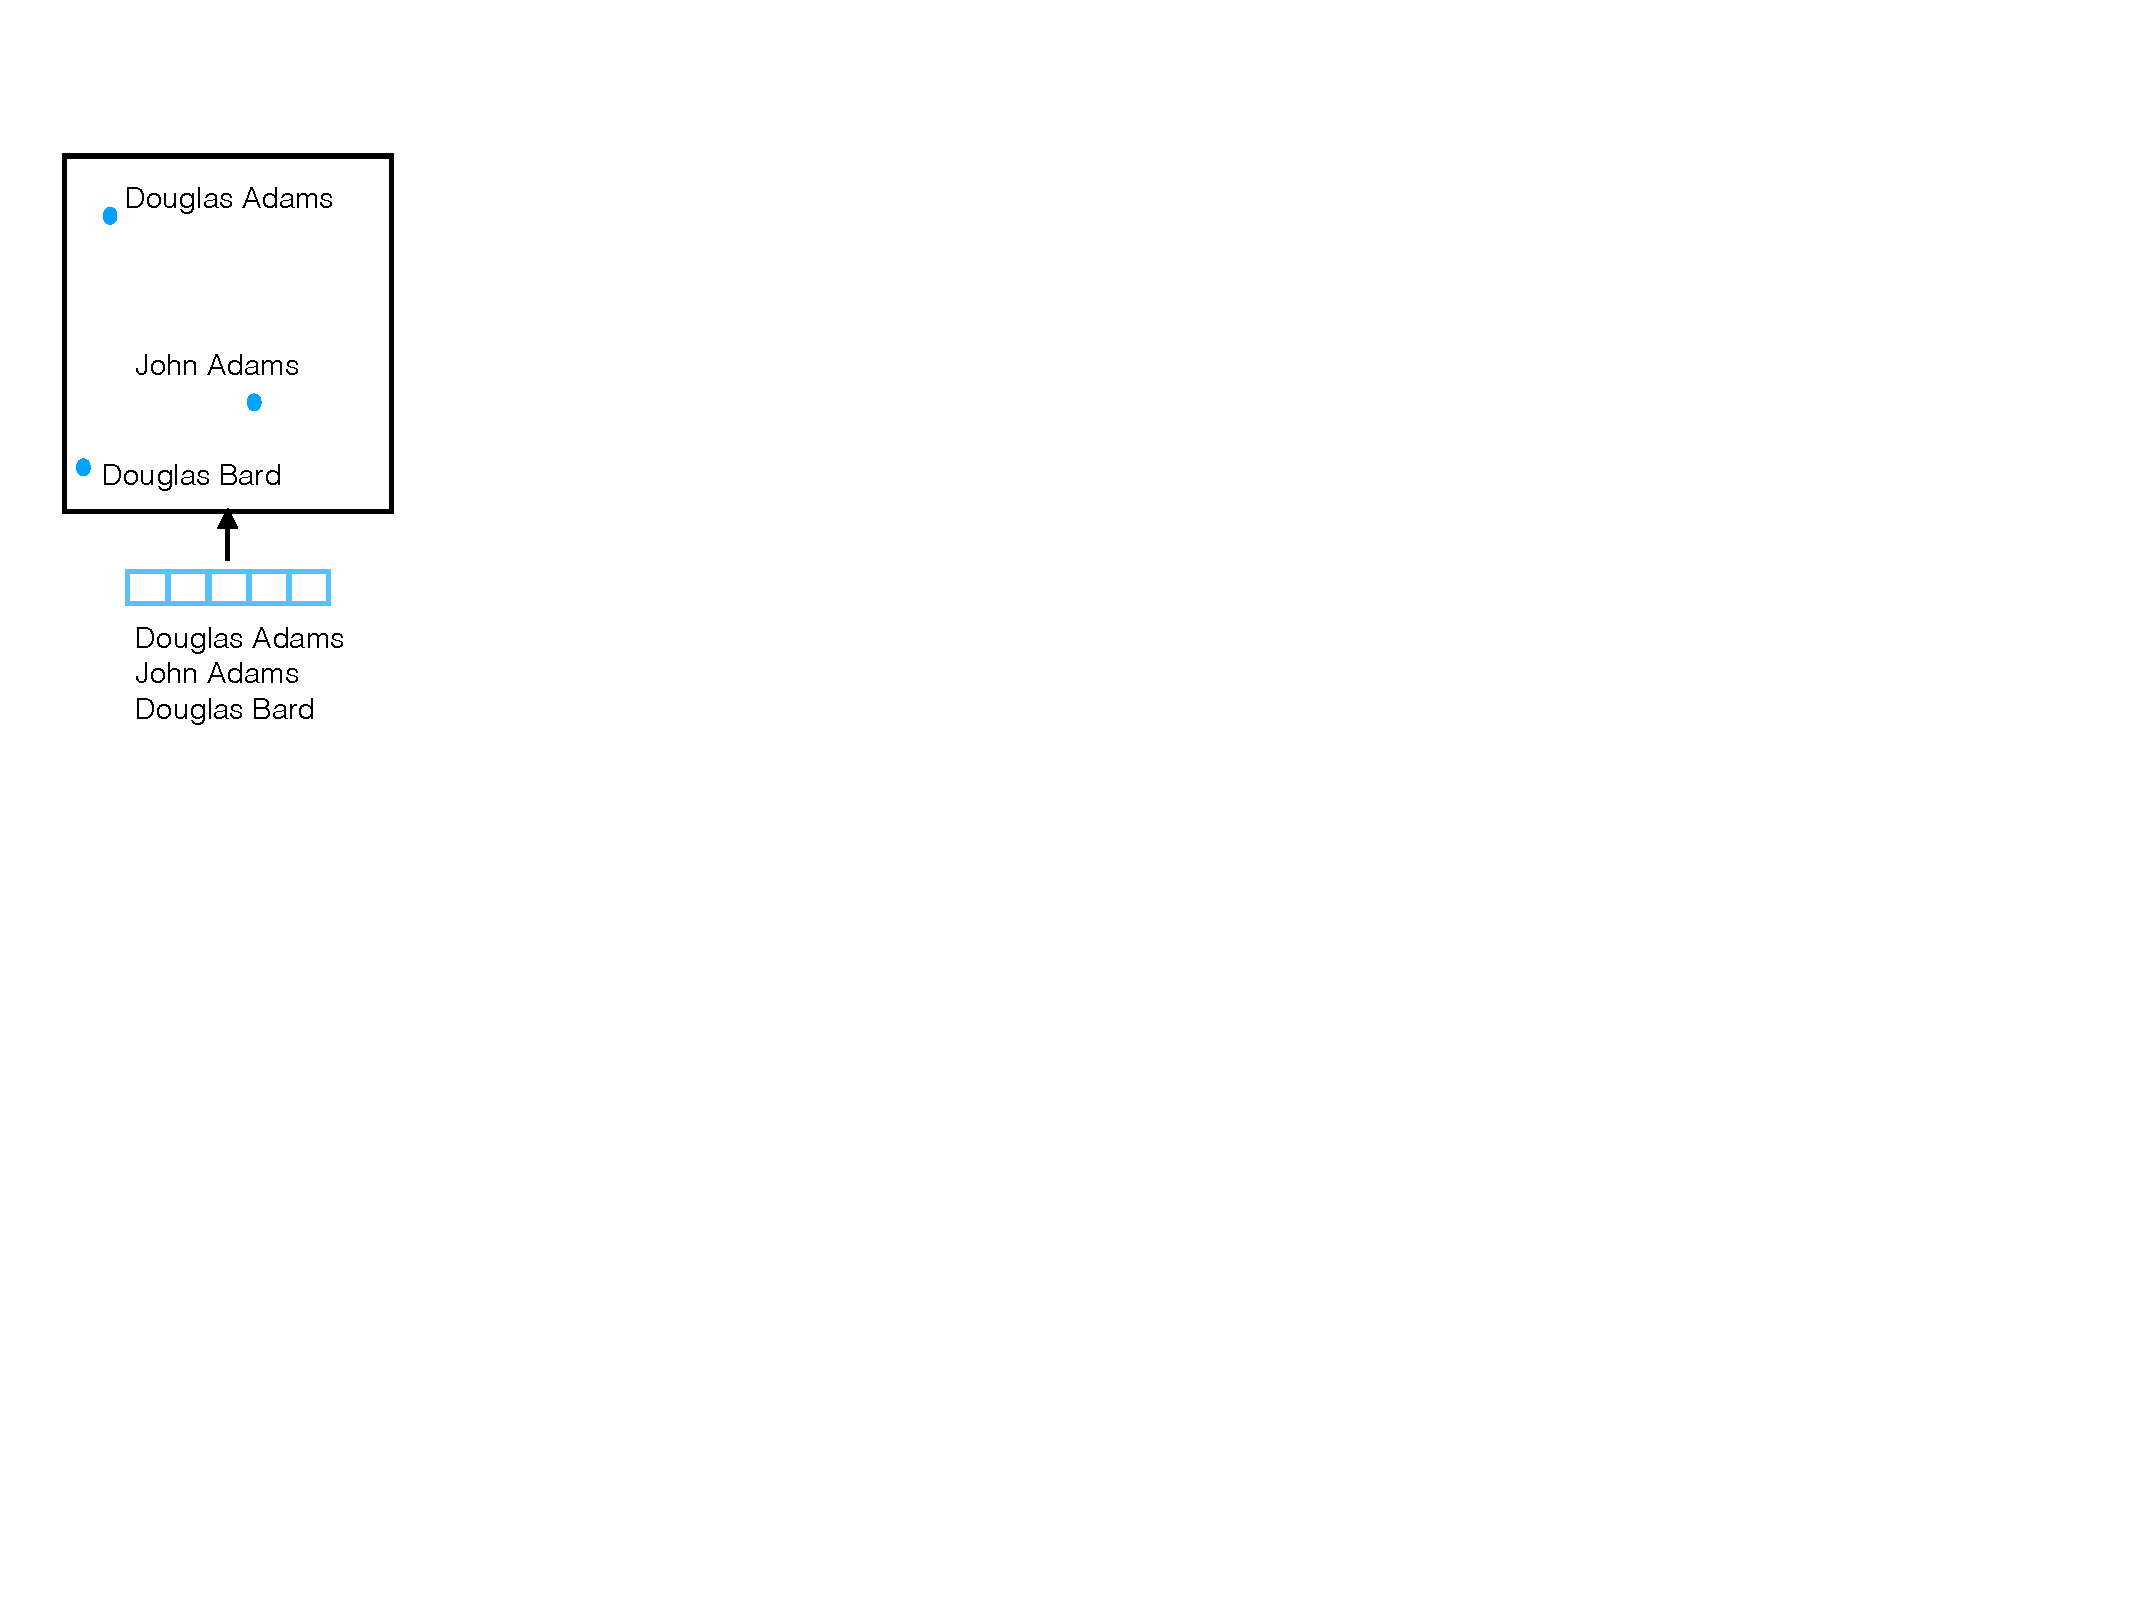
\includegraphics[width=.9\linewidth]{join3}
%        \caption{Index embeddings for left table's cell values in a nearest neighbors index}
%        \label{join3}
%    \end{subfigure}
%    ~ 
%    \begin{subfigure}[t]{0.24\linewidth}
%        \centering 
%        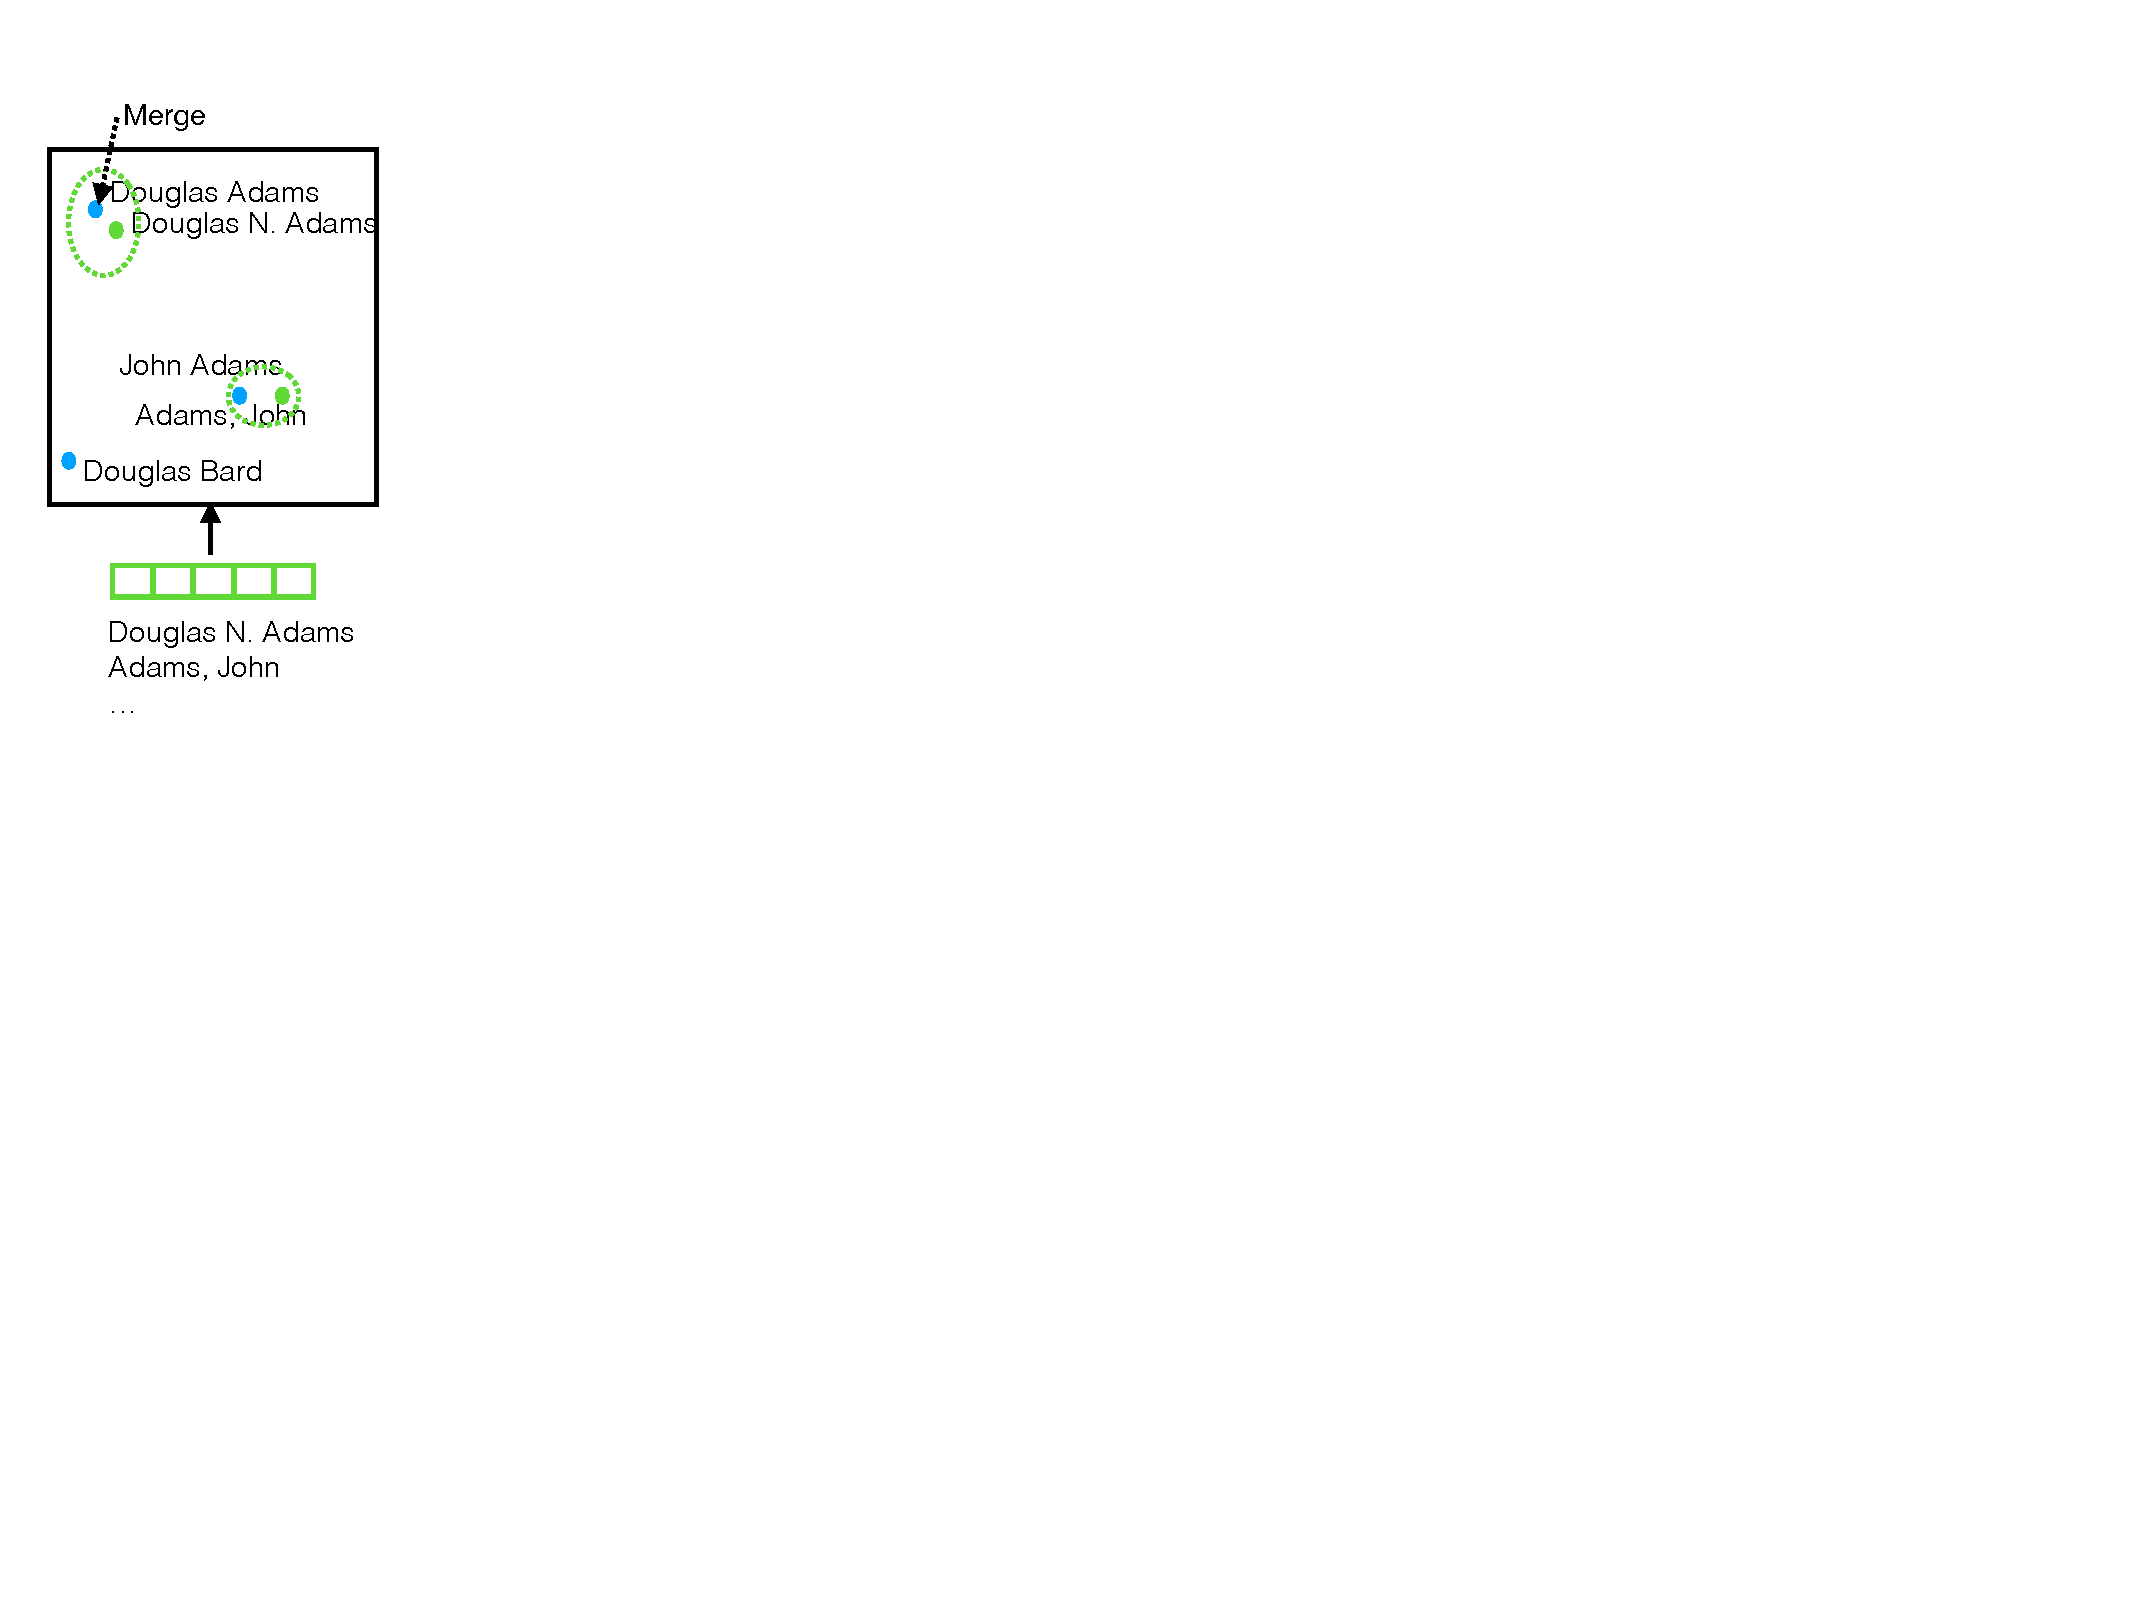
\includegraphics[width=.9\linewidth]{join4}
%        \caption{For each cell in right table, find closest neighbor(s) and merge these rows}
%        \label{join4}
%    \end{subfigure}
%    \caption{Overview of joins using deep learning}
%    \label{join_fig}
%\end{figure*}

Assuming we have deep learning models that are trained to produce the
right distance estimates for alternate surface forms for an entity,
the models can be used for a join as follows.  For each cell value in
the two columns to be joined, obtain vector embeddings from the last
layer of the network.  Note that although the siamese network has
three separate networks, each network is in fact identical to the
other two networks because they share weights.  For the left column
cell values, vector embeddings are inserted into an approximate
nearest neighbors index.  For each cell value in the right column,
vector embeddings are used as `query vectors' to query the approximate
nearest neighbors index.  In our context, merging the datasets would
involve joining the top $k$ rows in the left table that are `closest'
in distance to each cell value in the right table.  Note that the
choice of $k$ clearly has a direct effect on the tradeoff between
precision and recall, but for most practical uses of join, $k$ is
usually very small (typically 1).  This has implications on what
metrics we can use to evaluate joins, as we describe in our evaluation.

